\documentclass[aspectratio=169]{../latex_main/tntbeamer}  % you can pass all options of the beamer class, e.g., 'handout' or 'aspectratio=43'
\usepackage{dsfont}
\usepackage{bm}
\usepackage[english]{babel}
\usepackage[T1]{fontenc}
%\usepackage[utf8]{inputenc}
\usepackage{graphicx}
\graphicspath{ {./figures/} }
\usepackage{algorithm}
\usepackage[ruled,vlined,algo2e,linesnumbered]{algorithm2e}
\usepackage{hyperref}
\usepackage{booktabs}
\usepackage{mathtools}

\usepackage{amsmath,amssymb}

\DeclareMathOperator*{\argmax}{arg\,max}
\DeclareMathOperator*{\argmin}{arg\,min}

\usepackage{amsbsy}
\newcommand{\vect}[1]{\bm{#1}}
%\newcommand{\vect}[1]{\boldsymbol{#1}}

\usepackage{pgfplots}
\pgfplotsset{compat=1.16}
\usepackage{tikz}
\usetikzlibrary{trees} 
\usetikzlibrary{shapes.geometric}
\usetikzlibrary{positioning,shapes,shadows,arrows,calc,mindmap}
\usetikzlibrary{positioning,fadings,through}
\usetikzlibrary{decorations.pathreplacing}
\usetikzlibrary{intersections}
\pgfdeclarelayer{background}
\pgfdeclarelayer{foreground}
\pgfsetlayers{background,main,foreground}
\tikzstyle{activity}=[rectangle, draw=black, rounded corners, text centered, text width=8em]
\tikzstyle{data}=[rectangle, draw=black, text centered, text width=8em]
\tikzstyle{myarrow}=[->, thick, draw=black]

% Define the layers to draw the diagram
\pgfdeclarelayer{background}
\pgfdeclarelayer{foreground}
\pgfsetlayers{background,main,foreground}

% Requires XeLaTeX or LuaLaTeX
%\usepackage{unicode-math}

\usepackage{fontspec}
%\setsansfont{Arial}
\setsansfont{RotisSansSerifStd}[ 
Path=../latex_main/fonts/,
Extension = .otf,
UprightFont = *-Regular,  % or *-Light
BoldFont = *-ExtraBold,  % or *-Bold
ItalicFont = *-Italic
]
\setmonofont{Cascadia Mono}[
Scale=0.8
]

% scale factor adapted; mathrm font added (Benjamin Spitschan @TNT, 2021-06-01)
%\setmathfont[Scale=1.05]{Libertinus Math}
%\setmathrm[Scale=1.05]{Libertinus Math}

% other available math fonts are (not exhaustive)
% Latin Modern Math
% XITS Math
% Libertinus Math
% Asana Math
% Fira Math
% TeX Gyre Pagella Math
% TeX Gyre Bonum Math
% TeX Gyre Schola Math
% TeX Gyre Termes Math

% Literature References
\newcommand{\lit}[2]{\href{#2}{\footnotesize\color{black!60}[#1]}}

%%% Beamer Customization
%----------------------------------------------------------------------
% (Don't) Show sections in frame header. Options: 'sections', 'sections light', empty
\setbeamertemplate{headline}{empty}

% Add header logo for normal frames
\setheaderimage{
	% 
\includegraphics[height=\logoheight]{figures/TNT_darkv4.pdf}
	
\includegraphics[height=\logoheight]{../latex_main/figures/luh_logo_rgb_0_80_155.pdf}
	% 
\includegraphics[height=\logoheight]{figures/logo_tntluh.pdf}
}

% Header logo for title page
\settitleheaderimage{
	% 
\includegraphics[height=\logoheight]{figures/TNT_darkv4.pdf}
	
\includegraphics[height=\logoheight]{../latex_main/figures/luh_logo_rgb_0_80_155.pdf}
	% 
\includegraphics[height=\logoheight]{figures/logo_tntluh.pdf}
}

% Title page: tntdefault 
\setbeamertemplate{title page}[tntdefault]  % or luhstyle
% Add optional title image here
%\addtitlepageimagedefault{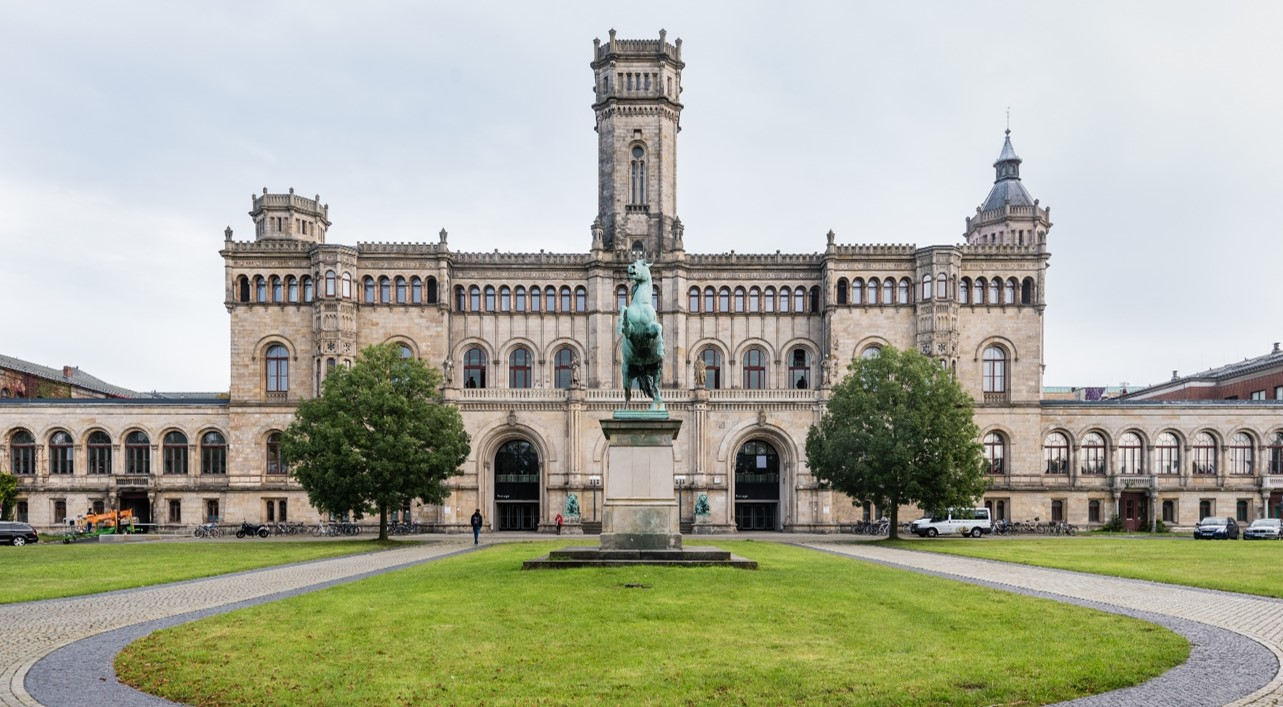
\includegraphics[width=0.65\textwidth]{figures/luh_default_presentation_title_image.jpg}}

% Title page: luhstyle
% \setbeamertemplate{title page}[luhstyle]
% % Add optional title image here
% \addtitlepageimage{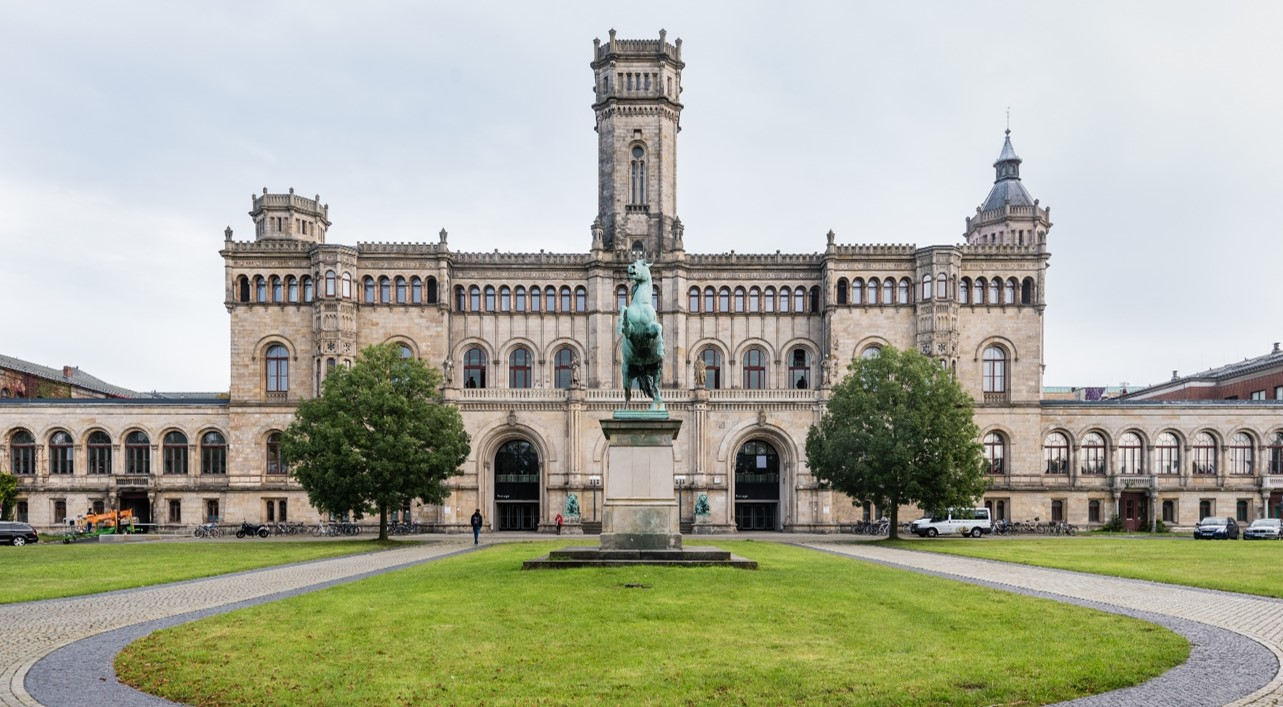
\includegraphics[width=0.75\textwidth]{figures/luh_default_presentation_title_image.jpg}}

\author[Abedjan \& Lindauer]{Ziawasch Abedjan \& Marius Lindauer\\[1em]
	
\includegraphics[height=\logoheight]{../latex_main/figures/luh_logo_rgb_0_80_155.pdf}\qquad
	
\includegraphics[height=\logoheight]{../latex_main/figures/DBIS_Kurzlogo.png}\qquad

\includegraphics[height=\logoheight]{../latex_main/figures/TNT_darkv4}\qquad

\includegraphics[height=\logoheight]{../latex_main/figures/L3S.jpg}	}
\date{Summer Term 2022; \hspace{0.5em} {
\includegraphics[height=1.5em]{../latex_main/figures/Cc-by-nc-sa_icon.svg.png}}; based on \href{https://ds100.org/fa21/}{[DS100]}
}


%%% Custom Packages
%----------------------------------------------------------------------
% Create dummy content
\usepackage{blindtext}

% Adds a frame with the current page layout. Just call \layout inside of a frame.
\usepackage{layout}


%%% Macros
%\renewcommand{\vec}[1]{\mathbf{#1}}
% \usepackage{bm}
%\let\vecb\bm

\title[Introduction]{DS: Introduction to Modeling}
\subtitle{Minimizing mean absolute error (MAE)}

\graphicspath{ {./figure/} }
%\institute{}


\begin{document}
	
	\maketitle
	\begin{frame}{Exploring MAE}
	    When we use absolute (or L1) loss, we call the average loss mean absolute error. For the constant model, our MAE looks like:
	    \begin{equation*}
	        R(\theta) = \frac{1}{n}\sum\limits_{i=1}^n|y_i - \theta|
	    \end{equation*}
	    Let’s again re-visit our toy example of 5 observations,  [20, 21, 22, 29, 33].
	    \begin{equation*}
	        L_1(20,\theta) = |20 - \theta| \hspace{1cm} R(\theta) = \frac{1}{5}(|20 - \theta| + |21-\theta| + |22 - \theta| + |29 - \theta| + |33 - \theta|)
	    \end{equation*}
	    \hspace{1cm}
\includegraphics[scale=.4]{Bild35}
	\end{frame}
	
	
	
	\begin{frame}{Exploring MSE}
	        $L_1(20,\theta) = |20 - \theta| \hspace{1cm} R(\theta) = \frac{1}{5}(|20 - \theta| + |21-\theta| + |22 - \theta| + |29 - \theta| + |33 - \theta|)$
	    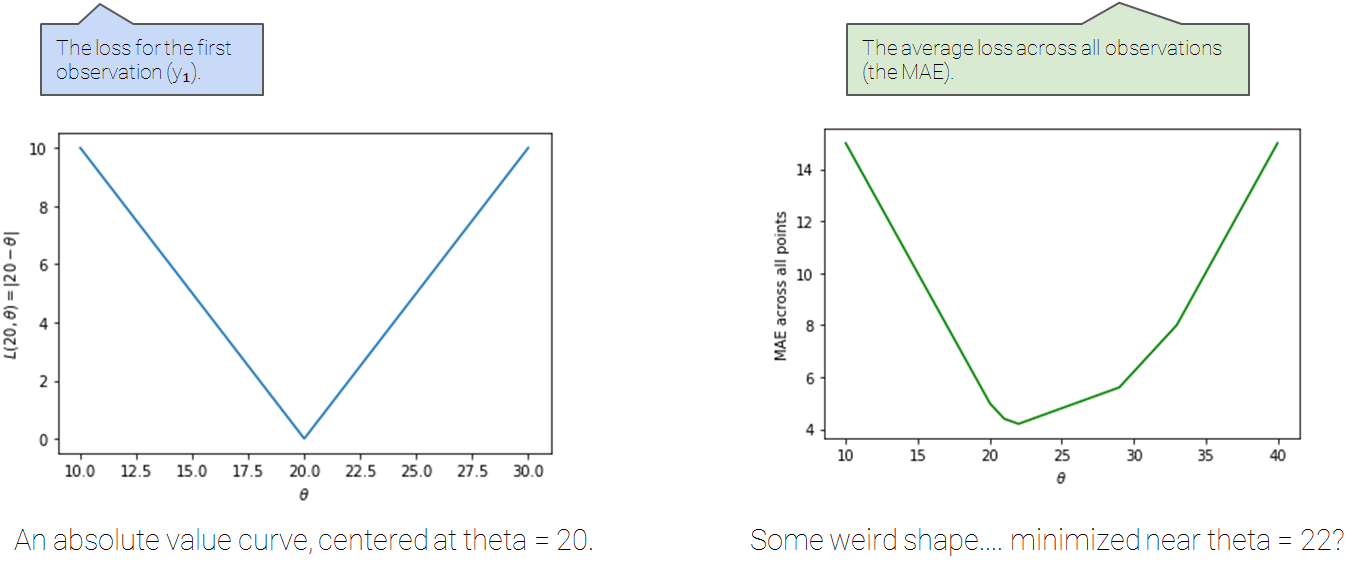
\includegraphics[scale=.4]{Bild36}
	\end{frame}
	
	
	\begin{frame}{Exploring MAE}
	    \begin{columns}
	        \begin{column}{.5\textwidth}
	                \\
	                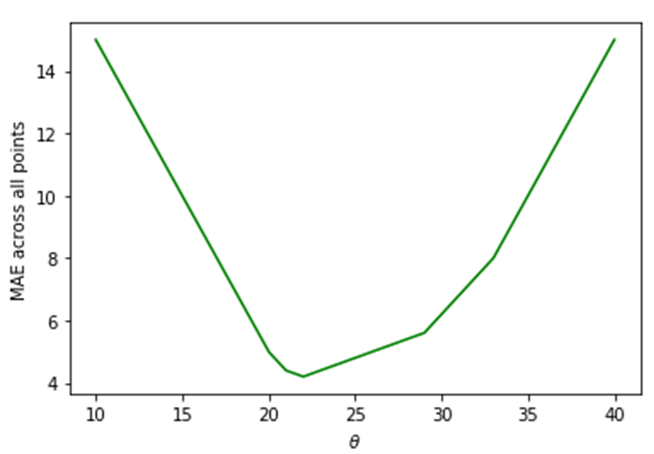
\includegraphics[scale=.4]{Bild37}
	        \end{column}
	        
	        
	        \begin{column}{.5\textwidth}
	                The shape of the MAE with the constant model seems to be jagged. This is because it is the (weighted) sum of several absolute value curves, which results in a piecewise linear function. \\
                    It also doesn’t seem to be immediately clear what the optimal choice of theta should be. It’s somewhere in the “middle” of our points, but it’s clearly not 25, which was the minimizing value for the MSE. \\
                    Let’s once again resort to calculus!
	        \end{column}
	    \end{columns}
	\end{frame}
	
	
	\begin{frame}{Exploring MAE}
	    \begin{columns}
	        \begin{column}{.5\textwidth}
	                \\
	                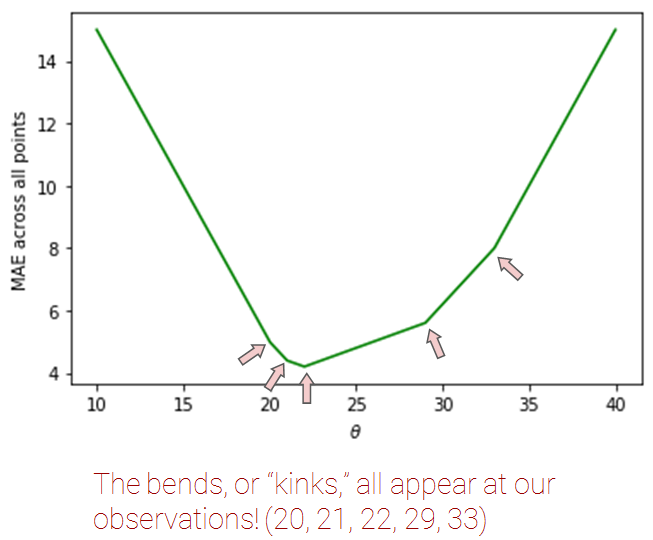
\includegraphics[scale=.4]{Bild38}
	        \end{column}
	        
	        
	        \begin{column}{.5\textwidth}
	                The shape of the MAE with the constant model seems to be jagged. This is because it is the (weighted) sum of several absolute value curves, which results in a piecewise linear function. \\
                    It also doesn’t seem to be immediately clear what the optimal choice of theta should be. It’s somewhere in the “middle” of our points, but it’s clearly not 25, which was the minimizing value for the MSE. \\
                    Let’s once again resort to calculus!
	        \end{column}
	    \end{columns}
	\end{frame}
	
	
	\begin{frame}{MAE minimization using calculus}
	    Once again, we can use calculus to determine the optimal  $\hat{\theta}$   .\\
        The first step is to determine the derivative of our loss function for a single point. Absolute value functions can be written as two piecewise linear functions:
        \begin{equation*}
            |y_i - \theta|  = \left\{\begin{array}{cc}
                y_i  - \theta & \text{if }\theta \leq y_i\\
               \theta - y_i  & \text{if } \theta > y_i
            \end{array}\right.
        \end{equation*}
        The derivative of our loss for a single point, then, is also a piecewise linear function:
        \begin{equation*}
            \frac{d}{d\theta}|y_i - \theta| = \left\{\begin{array}{cc}
               -1 & \text{if }\theta < y_i\\
              1  & \text{if } \theta > y_i
            \end{array}\right.
        \end{equation*}
        Note: The derivative of the absolute value when the argument is 0 (i.e. when          $y_i = \theta$   ) is technically undefined. We ignore this case in our derivation, since thankfully, it doesn’t change our result.      

	\end{frame}
	
	
	
	\begin{frame}{MAE minimization using calculus}
	    \begin{equation*}
            \frac{d}{d\theta}|y_i - \theta| = \left\{\begin{array}{cc}
               -1 & \text{if }\theta < y_i\\
              1  & \text{if } \theta > y_i
            \end{array}\right.
        \end{equation*}
        From here, we again use the fact that the derivative of a sum is a sum of derivatives:
        \begin{align*}
            \frac{d}{d\theta}R(\theta) &= \frac{1}{n}\sum\limits_{i=1}^n\frac{d}{d\theta}|y_i - \theta|\\
            &= \frac{1}{n}[\sum\limits_{\theta < y_i}(-1) + \sum\limits_{\theta > y_i} 1]
        \end{align*}\\
        
        \vspace{-.3cm}
        \hspace{2.5cm} 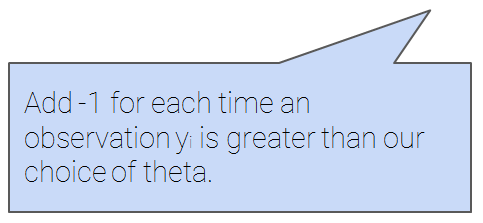
\includegraphics[scale=.4]{Bild39}\\
        \vspace{.3cm}
        
        
        \vspace{-2.8cm}
        \hspace{9.7cm} 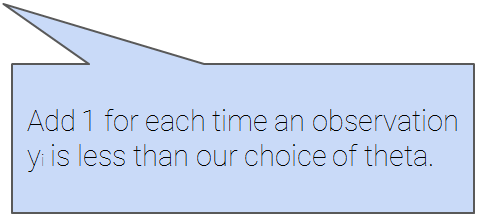
\includegraphics[scale=.4]{Bild40}\\
        \vspace{2.8cm}
	\end{frame}
	
	
	\begin{frame}{MAE minimization using calculus}
	    Setting this derivative equal to 0:
	    \begin{align*}
	        0 &= \frac{1}{n}[\sum\limits_{\theta < y_i} (-1) + \sum\limits_{\theta > y_i} 1 ]\\
	        0 &= - \sum\limits_{\theta < y_i} 1 + \sum\limits_{\theta > y_i} 1\\
	        \sum\limits_{\theta < y_i} 1 &= \sum\limits_{\theta > y_i} 1
	    \end{align*}
	    The last line is telling us that in order for our MAE to be minimized, we need to choose a theta such that the number of observations less than theta needs to be equal to the number of observations greater than theta.

	\end{frame}
	
	
	
	\begin{frame}{MAE minimization using calculus}
	    \begin{align*}
	        \sum\limits_{\theta < y_i} 1 &= \sum\limits_{\theta > y_i} 1
	    \end{align*}
	    In order for our MAE to be minimized, we need to choose a theta such that the number of observations less than theta needs to be equal to the number of observations greater than theta. In other words, theta needs to be such that there are an equal number of points to the left and right.\\
	    \bigskip
	    This is the definition of the median! For example, in our toy dataset, the point below in red (22) is the median of our observations. It is the value in the “middle.”\\
	    \hspace{4cm} 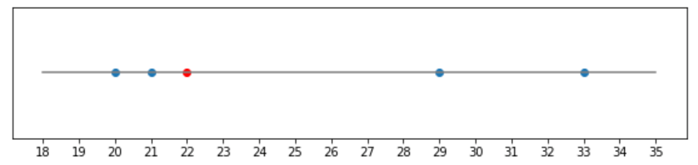
\includegraphics[scale=.5]{Bild41}
	\end{frame}
	
	
	\begin{frame}{MAE minimization using calculus}
	    \begin{align*}
	        \sum\limits_{\theta < y_i} 1 &= \sum\limits_{\theta > y_i} 1
	    \end{align*}
	    In order for our MAE to be minimized, we need to choose a theta such that the number of observations less than theta needs to be equal to the number of observations greater than theta. In other words, theta needs to be such that there are an equal number of points to the left and right.\\
	    \bigskip
	    This is the definition of the median! For example, in our toy dataset, the point below in red (22) is the median of our observations. It is the value in the “middle.”\\
	    \hspace{4cm} 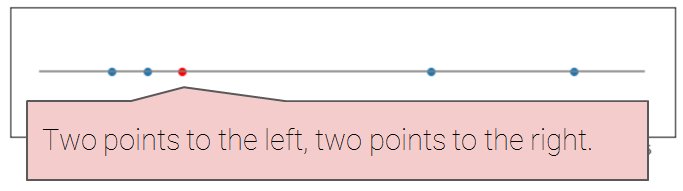
\includegraphics[scale=.4]{Bild42}
	\end{frame}
	
	
	\begin{frame}{Median minimizes MAE for the constant model}
	    We’ve now shown that the median minimizes MAE for the constant model.
	    \begin{equation*}
	        \hat{\theta} = \text{median}(y)
	    \end{equation*}
	    This is consistent with what we saw earlier, when plotting the MAE for our toy dataset: 
	    \begin{columns}
	        \begin{column}{.5\textwidth}
	                \\
	                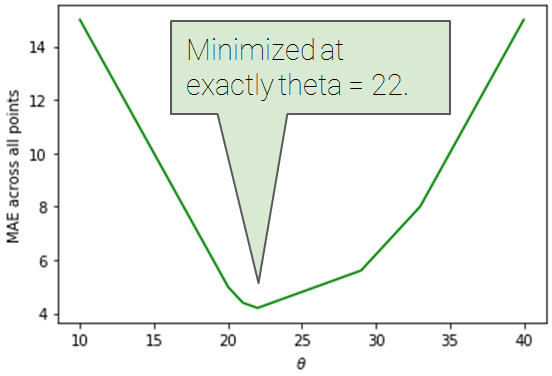
\includegraphics[scale=.4]{Bild43}
	        \end{column}
	        
	        
	        \begin{column}{.5\textwidth}
	              \vspace{.2cm}\\
	              Important note: In general, the mean and median of a dataset are not the same. Therefore, using MSE and MAE give us different optimal theta values! \\
                  A key takeaway here is that our choice of loss function determines the optimal parameters for our model.
  
	        \end{column}
	    \end{columns}
	\end{frame}
	
	
	
	\begin{frame}{Median minimizes MAE for the constant model}
	    \begin{columns}
	        \begin{column}{.6\textwidth}
	                \\
	                 Our toy dataset only had 5 observations. What if it had an even number of observations? Let’s say our toy dataset is now [20, 21, 22, 29, 33, 35]. The 35 is new.
	                 \begin{itemize}
	                     \item There’s no longer a unique solution!
	                     \item Any value in the range [22, 29] minimizes MAE.
	                     \item This reflects the fact that there are an even number of observations, and any number in that range has the same number of points to the left and right.
	                     \item (When there are an even number of data points, we typically set the median to be the mean of the two middle ones. Here, that’d be 25.5.)
	                 \end{itemize}
	        \end{column}
	        
	        
	        \begin{column}{.4\textwidth}
	              \\
	              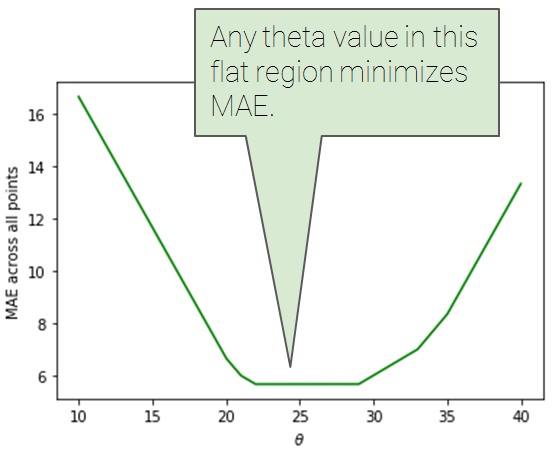
\includegraphics[scale=.4]{Bild44}
  
	        \end{column}
	    \end{columns}
	\end{frame}
\end{document}